% This is a simple sample document.  For more complicated documents take a look in the exercise tab. Note that everything that comes after a % symbol is treated as comment and ignored when the code is compiled.

\documentclass[12pt]{article} % \documentclass{} is the first command in any LaTeX code.  It is used to define what kind of document you are creating such as an article or a book, and begins the document preamble
\usepackage{amssymb}
\usepackage[utf8]{inputenc}
\usepackage{glossaries}


\makeglossaries

\newglossaryentry{SolCor}{
	name={couronne solaire},
	description={l'atmosphère du soleil}
}

\newglossaryentry{SolVoil}{
	name={voile solaire},
	description={une méthode de propulsion experimentale utilisant la pression solaire pour avancer, genère des forces extremement faibles mais ne coûte pas de carburant}
}

\newglossaryentry{Elec}{
name={moteur ionique},
description={un moteur fusée propulsant de petites quantités de matières à très grande vitesses à l'aide d'électricité générant ainsi des poussées très faibles mais très efficaces (peu coûteuse en carburant)}
}


\newglossaryentry{Zone}{
	name={zone d'observation},
	description={région dans laquelle le soleil est intégrallement caché pas l'objet occultant mais où l'intégralité de la couronne est visible, ici l'astre occultant sera toujours la Lune}
}

\newglossaryentry{Obs}{
	name={observation},
	description={correspond à une trajectoire passive (sans contrôle) durant laquelle l'objet se situe dans la zone d'observation, une observation commence lorsque l'objet entre dans la zone et s'arrête quand il en sort}
}

\newglossaryentry{AscObs}{
	name={observation ascendante},
	description={observation type assez longue ayant lieu entre le premier croissant et le premier quartier de la Lune, durant l'observation l'objet s'éloigne de la Terre.}
}

\newglossaryentry{DesObs}{
	name={observation descendante},
	description={observation type assez longue ayant lieu entre le dernier quartier et le dernier croissant de la Lune, durant l'observation l'objet se rapproche de la Terre.}
}


\newglossaryentry{Cont}{
	name={contrôle},
	description={dans un problème de contrôle optimal le contrôle est une fonction qui dépend de l'état et du temps qui influence la dynamique d'un système, dans le cadre de ce stage, le contrôle est une fonction qui indique un vecteur 3D en fonction du temps}
}

\newglossaryentry{Cor}{
	name={coronographe},
	description={un téléscope équipé d'un disque opaque cachant la partie la plus lumineuse de l'objet observé permettant d'observer les détails les moins lumineux, utilisé majoritairement pour observer la couronne solaire d'où son  nom}
}


\usepackage{amsmath} % \usepackage is a command that allows you to add functionality to your LaTeX code
\usepackage[left=2cm, right=2cm,bottom=2.5cm]{geometry}
\title{Rapport de Stage} % Sets article title
\author{Vincent Callegari} % Sets authors name
\date{\today} % Sets date for date compiled
\usepackage{graphicx}


\usepackage{float}








\graphicspath{{./images/graph/}}
% The preamble ends with the command \begin{document}
	\begin{document}
		\maketitle
		\includegraphics[width=1\textwidth]{images/eclipse_2.png}
		\vfill
		
\includegraphics[width=3cm]{images/Logo_Reseau_Polytech.png} \hfill 
\includegraphics[width=3cm]{images/inria.png}
		\newpage
		\tableofcontents
		\newpage
		\section{Introduction}
		
		\subsection{La problèmatique}
		Le but de ce stage est de d'étudier une mission spatiale visant à étudier la \gls{SolCor} en utilisant la Lune comme corps occultant. En outre l'objectif est de calculer des trajectoires optimales faisable par des satellite exerçant des poussées faible (par \gls{Elec} ou \gls{SolVoil}).
		
		La voile solaire fonctionne de la même manière qu'une voile normale à l'exception qu'elle utilise la quantité de mouvement de la lumière au lieu de la quantité de mouvement de l'air pour changer de vitesse. Les forces générées par des voiles solaires ne peuvent pas être dirigées dans toutes les directions et sont très faibles en comparaison d'autres formes de propulsions les plus utilisés par les véhicules spatiaux mais ont le grand avantage de ne pas dépenser de carburant.
		
		La propulsion électrique quand à elle utilise un champ magnétique pour accélérer un gaz ionisé (souvent un gaz noble comme le xénon par exemple), l'idée est de créer une propulsion extrêmement efficace grâce à la vitesses très élevé des particules permettant ainsi de faire gagner une grande vitesse au satellite pour une masse de carburant relativement faible. Le désavantage de cette méthode de propulsion est qu'elle ne permet pas de générer de grandes forces de poussée ce qui signifie qu'elle ne peut pas être utilisée avec des vaisseaux trop lourds ou pour le décollage de fusées.
		
		La couronne solaire (aussi appelé chromosphère) est en quelque sorte l'atmosphère du soleil, c'est une des parties du soleil qui est la plus mal comprise, on sait que c'est ici que se manifestent des événements violent comme les éruptions solaires ce qui influence la climat terrestre. Essayer de mieux comprendre le fonctionnement de la couronne solaire est donc un objectif assez important des astronomes.
		
		L'observation de la couronne solaire est un tâche difficile car elle est bien moins lumineuse que le soleil lui même. Afin d'observer cette couronne, il est donc nécessaire d'occulter le disque solaire.
		
		Sur Terre il est possible d'effectuer des observations de la couronne solaire durant les éclipses totales où la Lune joue le rôle d'objet occultant. Cependant ces observations ont lieu en moyenne une fois tout les 18 mois et ne permettent des observations de quelques minutes à peine ce qui n'est pas idéal.
		
		une autres méthode pour effectuer d'effectuer de telles observations en utilisant un \gls{Cor} qui utilise un masque pour cacher la partie la plus lumineuse du Soleil. Cependant plus l'objet utilisé pour occulter le Soleil est grand et éloigné, plus l'observation peut être précise. Les planètes, planètes naines et autre astres sphériques opaques sont donc des objets idéaux pour effectuer des mesures car leurs taille excède largement tout objets occultant que l'humanité peut construire à ce jour. De plus, comme c'est souvent le cas en astronomie, l'atmosphère terrestre est souvent un obstacle pour effectuer des observations, particulièrement de jour.
		
		L'objet du système solaire qui semble le plus indiqué pour être utilisé comme astre occultant est la Lune car son absence d'atmosphère et sa grande proximité avec la Terre combiné avec sa petite taille permettent d'effectuer des observations à distance relativement faible (environ égale à la distance Terre-Lune) tout en ayant les avantages énoncé plus tôt.
		 
		La contrepartie lorsque l'on utilise une planète comme objet occultant est qu'on ne peut contrôler sa trajectoire et que le satellite est contraint de suivre l'objet, ce qui demande de résoudre un certain nombres de problèmes et de se plier à un certain nombre de contraintes.
		
		Ainsi l'objectif de mon stage est d'étudier les possibilités d'effectuer des observations de la couronne solaire en utilisant la Lune comme objet occultant.
		 
		Dans ce rapport, je vais détailler le travail que j'ai effectué et les conclusions et résultats auxquels je suis arrivé ainsi que les compétence acquise au cours du stage. 
		 
		\subsection{Institut de recherche}
		
		l'Institut national de recherche en informatique et en automatique (INRIA) est un laboratoire publique de recherche. Il est implémenté dans sur nombreux sites :  Bordeaux, Grenoble, Lille, Lyon, Lorraine, Paris, Rennes, Saclay, Côte d'Azur et le Chesnay. J'ai effectué mon stage sur le site de Sophia Antipolis (Alpes Maritimes). Le laboratoire à été fondée en 1967 (il s'appelait alors seulement l'Institut de recherche en informatique et en automatique ou IRIA) dans le cadre de l'initiative du plan Calcul visant à s'assurer que la France conserve une indépendance en innovation informatique.
		
		
		\newpage
		\section{Travail demandé}
		\subsection{Objectif du stage}
		Le travail qui m'a été demandé durant ce stage regroupait plusieurs tâches : tout d'abord, étudier la géométrie de la \gls{Zone} au cours du temps (la zone d'observation étant la région où le soleil est caché par la lune mais où la couronne solaire reste visible). Ensuite il fallait, à partir de ces résultats, essayer de trouver des trajectoires permettant de traverser la zone d'observation de manière répété et ensuite de maximiser le temps d'observation.
		
		Plusieurs corps célestes seront considéré dans l'étude de ce problème : Le Soleil, La Terre et la Lune. Il s'agit donc d'un problème à quatre corps (les trois énoncé plus tôt en plus du satellite). Dans ce contexte il est presque impossible de trouver une trajectoire passive (sans \gls{Cont}) permettant de faire des observations répété. Ainsi il est nécessaire d'ajouter un contrôle au système c'est à dire ajouter un système de propulsion au satellite. Il était initialement prévu d'utiliser une \gls{SolVoil} comme méthode de propulsion mais il s'aggrave plus pratique d'utiliser un \gls{Elec}.
			
		%Étant donné qu'il y aura sans doute de nombreuses forces perturbatrices et qu'une trajectoire passive (un objet sans contrôle qui ne subit que les forces de gravité de la Terre, Lune, Soleil etc ...) ne traversera sans doute pas la zone d'observation très souvent, il est nécessaire d'ajouter au système un contrôle pour corriger la trajectoire du satellite voire de la changer. le système de propulsion qui à été choisi pour accomplir cet objectif est une voile solaire. Il s'agit d'un problème de contrôle optimal ce qui signifie que j'ai du en apprendre plus sur dans ce domaine car je n'ai pas encore suivi les cours sur ce sujet.
		
		Le but final du projet est de présenter un rapport final rapportant tous les résultats et observations faîtes lors du stages ainsi que des programmes capable de calculer différentes valeur utile (zone d'observation, trajectoire de satellite ou contrôle de ce dernier).
		
		\subsection{tâches}
		En résumé mon travail se répartit en plusieurs étapes décrite ci après:
		\begin{itemize}
			\item Calculer la géométrie de la \gls{Zone};
			\item Trouver des trajectoires passive (sans contrôle) qui permettent des \glspl{Obs};
			\item Trouver des trajectoires active (avec contrôle) qui permettent des observations répétés;
			\item Résumer tous les résultats dans un rapport en anglais.
		\end{itemize}
		
		Calculer les trajectoires de la \gls{Zone} demandera dans un premier temps d'étudier de la littérature scientifique en rapport avec ce thème. Il faudra ensuite mettre au point d'un bon modèle mathématique pour définir la géométrie de la zone d'observation ainsi qu'un modèle pour définir le problème. Pour cela il faudra évidement trouver une méthode qui permet de déterminer si un objet est dans la zone d'observation.
		\\ \\
		L'étape suivante consiste à trouver des trajectoires passives (c'est à dire sans \gls{Cont}). Pour cela il faudra implémenter un programme qui simulera la dynamique de l'objet ainsi qu'une méthode adapté pour évaluer des trajectoires effectuant des observations. Cette étape permettra de déterminer la forme générale  des \glspl{Obs} intéressantes ce qui sera utile pour l'étape suivante.
		\\ \\
		Par la suite il faudra ajouter un contrôle dans l'optique de maximiser le nombre d'observations. Pour cela il faudra modifier le code déjà existant ou en créer un nouveau. C'est à ce moment là que l'on pourra obtenir une réponse sur la possibilité d'utiliser une voile solaire et les solutions alternative.
		\\ \\
		Pour finir il faudra résumer tout le travail et tous les résultats obtenu dans un rapport rédigé en anglais ainsi que rendre les programmes informatique produits lisible et clair dans l'optique d'utilisations futures de ces codes par des personnes potentiellement étrangères au projet.
		\\ \\
		%De plus le modèle utilisé pour résoudre ce problème sera d'abord implémenté dans une version simplifiée : simple trajectoire circulaire de la lune avec vitesse fixe en 2D. Puis gagneras en complexité au fur et à mesure que le projet avanceras jusqu'à être très proche de la réalité (prise en compte de la variation de l'orbite lunaire causé par le soleil par exemple).
		
		\newpage
		\section{Travail effectué}
		
		\subsection{Première observations}
		Avant de commencer à travailler sur le problème, il fallait que j'en apprenne plus sur les notions du projet, j'ai donc lu divers articles qui m'ont été fourni. Il y avait des articles sur des projets d'occultation solaire à l'aide de la Terre (utilisée comme astre occultant), une thèse sur les voiles solaires, ainsi qu'un cours sur le contrôle optimal car je n'ai pas encore eu de cours sur ce sujet.
		
		J'ai ensuite analysé le déplacement de la \gls{Zone} de la Lune. J'ai utilisé des notions basiques de géométrie pour déterminer où se trouvait la zone d'observation de la Lune en fonction de sa position.
		
		La forme de la zone d'observation dépend de la taille de l'objet occultant (ici la Lune), de la distance entre le Soleil et l'objet (ici environ la distance Terre-Soleil soit environ 150 millions de Km) ainsi que de la précision de l'observation. En effet plus on souhaite observer des partie de la couronne proche du soleil plus la zone d'observation sera réduite car il faudra être plus proche du point où le Soleil est exactement caché par l'astre occultant sans que cet astre cache la zone périphérique du soleil. Cette valeur est définie par un pourcentage du rayon solaire appelé $\alpha$, une valeur de $\alpha$ de $5\%$ par exemple signifie que l'on tolère de que des parties de la couronne solaire étant à moins de $0.05$ rayon solaire de la surface soir caché par l'astre occultant.
		
		la forme de la zone d'observation est l'intersection de deux cônes : le cône dans lequel la couronne solaire est visible (en prenant en compte la tolérance $\alpha$). et le cône dans lequel le soleil est caché.
		
		\begin{figure}[H]
			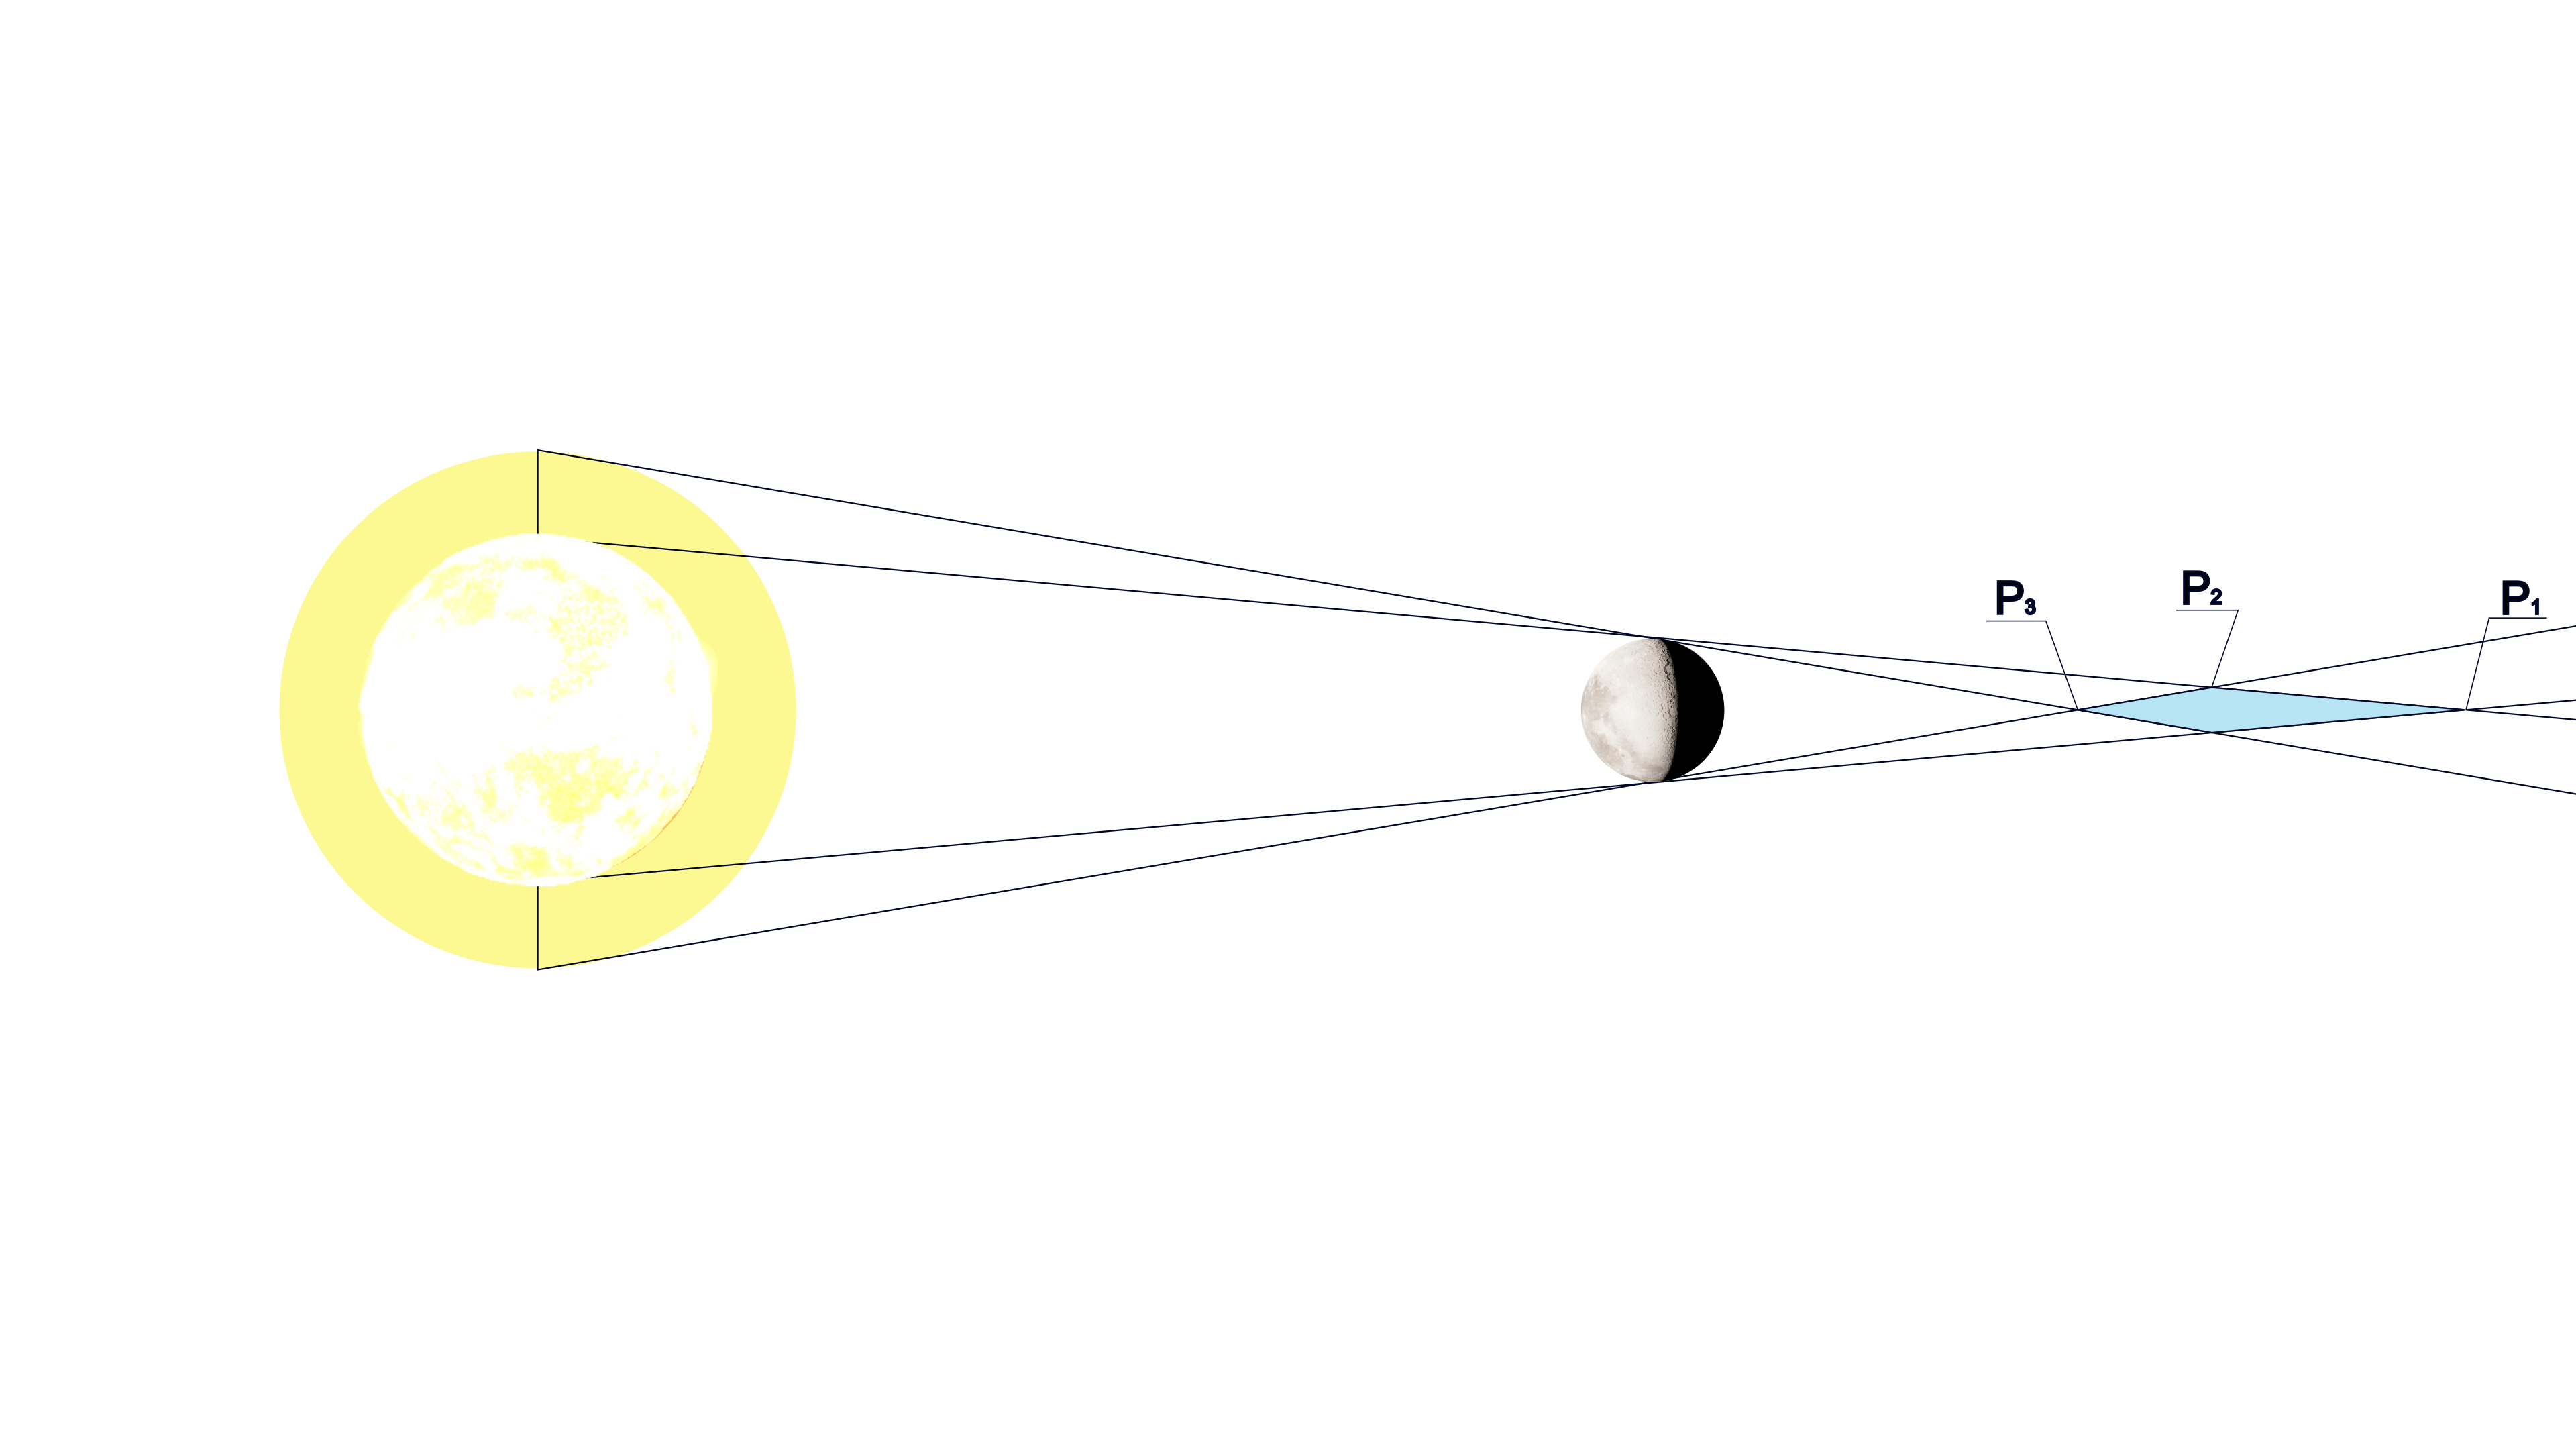
\includegraphics[width=1\textwidth]{images/moon_schem.png}
			\caption{géométrie de la zone d'observation}
		\end{figure}
		
		J'ai obtenu les formules suivantes pour les positions des points $P_1$, $P_2$ et $P_3$ relativement à la Lune quand elle est à une distance $D$ du Soleil (voir figure 1).
		
		$$	
		P_{1x}=\frac{\bar{D}R_l}{R_s-R_l}
		$$ 
		$$	
		P_{3x}=\frac{\bar{D}R_l}{R_s(\alpha+1)-R_l}
		$$
		$$
		P_{2x}=\frac{P_{1x}tan(\theta_1) + P_{3x}tan(\theta_3)}{tan(\theta_1) + tan(\theta_3)}
		$$
		$$
		P_{2y}=tan(\theta_1)(P_{1x}-P_{2x})
		$$
		
		avec
		$$
		\theta_1=\sin^{-1}\left(\frac{R_l}{P_{1x}}\right)
		$$
		
		$$
		\theta_3=\sin^{-1}\left(\frac{R_l}{P_{3x}}\right)
		$$
		
		A partir de ces valeurs il est possible de déterminer les positions des points $P_1$ et $P_3$ où que soit la Lune à l'aide simple produit en croix.
		
		$$
		\begin{equation}
			P_3=R_{lt}+\hat{P_{3x}}D^{-1}R_{ls} 
		\end{equation}
		$$
		$$
		\begin{equation}
			P_1=R_{lt}+\hat{P_{1x}}D^{-1}R_{ls} 
		\end{equation}
		$$
		
		La position du point $P_2$ est approximée pour réduire les calculs. J'ai choisi d'utiliser cette méthode approchée pour évaluer la zone d'observation pour essayer de réduire le coût de calcul. Cela permettra d'accélérer l'exécution du code qui sera implémenté plus tard car cette opération sera répétée extrêmement souvent.
		
		En prenant $D$ égal à la distance Terre soleil, j'ai calculé qu'on obtient une erreur de l'ordre de quelques centaines de mètres sur la position du point $P_2$ ce qui est négligeable en comparaison de l'épaisseur de la zone d'observation.
		
		Pour une valeur de $\alpha$ de $5\%$ la zone d'observation à une longueur d'environ $18000 Km$ pour une épaisseur d'environs $85 Km$. On peut ainsi voir que la zone d'observation est extrêmement fine.
		
		Après avoir utilisé des outils graphiques pour visualiser clairement la forme de la \gls{Zone} et avoir déjà calculé à la main des candidats d'\gls{Obs} qui semblait être intéressante j'ai recherché une bonne méthode pour évaluer des trajectoires.
		
		Concernant la dynamique du système les états (positions et vitesses) de la Terre et de la Lune sont calculé dans un système à 3 corps avec le Soleil fixé à l'origine. De cette manière on n'aura besoin de calculer les états de la Lune et de la Terre qu'une seule fois au début du calcul. Une fois ce système résolu la dynamique du satellite est calculé avec les équations suivantes dans le référentiel du centre de gravité du système Terre-Lune :
		
		$$
		\begin{bmatrix}
			\dot{\overrightarrow{R_{s}}}\\
			\dot{\overrightarrow{V_{s}}}\\
		\end{bmatrix} =\begin{bmatrix}
			\overrightarrow{V_{s}}\\
			G_{m}(R_s,R_m)+G_{t}(R_s,R_t)
		\end{bmatrix}
		$$
		
		avec $G_m$ et $G_t$ respectivement la force de gravité lunaire et la force de gravité terrestre. Notez que la gravité solaire ne figure pas dans l'équation car on se place dans le référentiel du système Terre-Lune (bien qu'il faudrait techniquement prendre en compte la très légère variation de la force de gravité solaire). Dans cette équation le satellite n'a pas de contrôle car il ne peut pas à la fois observer et changer sa trajectoire.
		
		\subsection{Calcul des observations}
		Une fois cette étape théorique passé, j'ai implémenté le modèle dans Matlab ainsi qu'une méthode permettant de calculer le temps passé dans la \gls{Zone} en fonction d'une vitesse et position initiale situé dans la zone d'observation, De part la longueur importante de cette dernière, j'ai choisis de simplifier la position initiale du satellite par une ligne reliant les points $P_1$ et $P_3$. La méthode permettant de calculer le temps passé dans la zone simule la dynamique du système avant et après la position initiale pour déterminer l'instant où l'objet entre dans la zone et l'instant où ce dernier en sort ce qui permet de calculer le temps d'observation. L'objectif du problème est de maximiser le temps passé dans la zone d'observation lors de cette observation uniquement. Ce choix à été fait car j'ai remarqué qu'il y avait quelques points précis qui permettaient des temps d'observation extrêmement long (plus de 15 heures) par rapport aux temps d'observation médian (quelques minutes) ce qui m'a fait penser qu'il serait sans doute inutile de chercher des orbites permettant plusieurs observations quand une seule de ces longues observations serait meilleure en tout point.
		\\ \\
		J'ai pu obtenir de premiers résultat consistant simplement à fixer tout les paramètres sauf un et d'afficher dans un graphe les variations causée. Ces résultats ont permis de mettre en évidence deux points de l'orbite lunaire qui semblait être assez intéressants pour effectuer des observations : ces deux points se situent aux moments où le Soleil, la Terre et la Lune forment un angle d'environs 60 degrés (\gls{AscObs} et \gls{DesObs}). Du point de vue de la Terre cela représente les moments où un tiers de la Lune est illuminé par le Soleil. le satellite se situerais aussi sur l'orbite de la Lune mais 60 degrés plus loin (le Soleil, la Terre et le satellite formerais donc un angle de 120 degrés) mais se déplacerait dans la même direction que la Lune afin d'accompagner la zone d'observation (voir figure 2). Il faut noter cependant que ces résultats sont valables dans un modèle très simplifié (orbite lunaire ronde, soleil fixe, distance de la zone d'observation exactement égale au rayon de l'orbite lunaire etc...), les vrais résultats ont des orbites assez similaires mais de nombreux facteurs font que les valeurs optimales ne correspondent pas exactement à ce qui est énoncé ci dessus.
		
		
		\begin{figure}[h]
			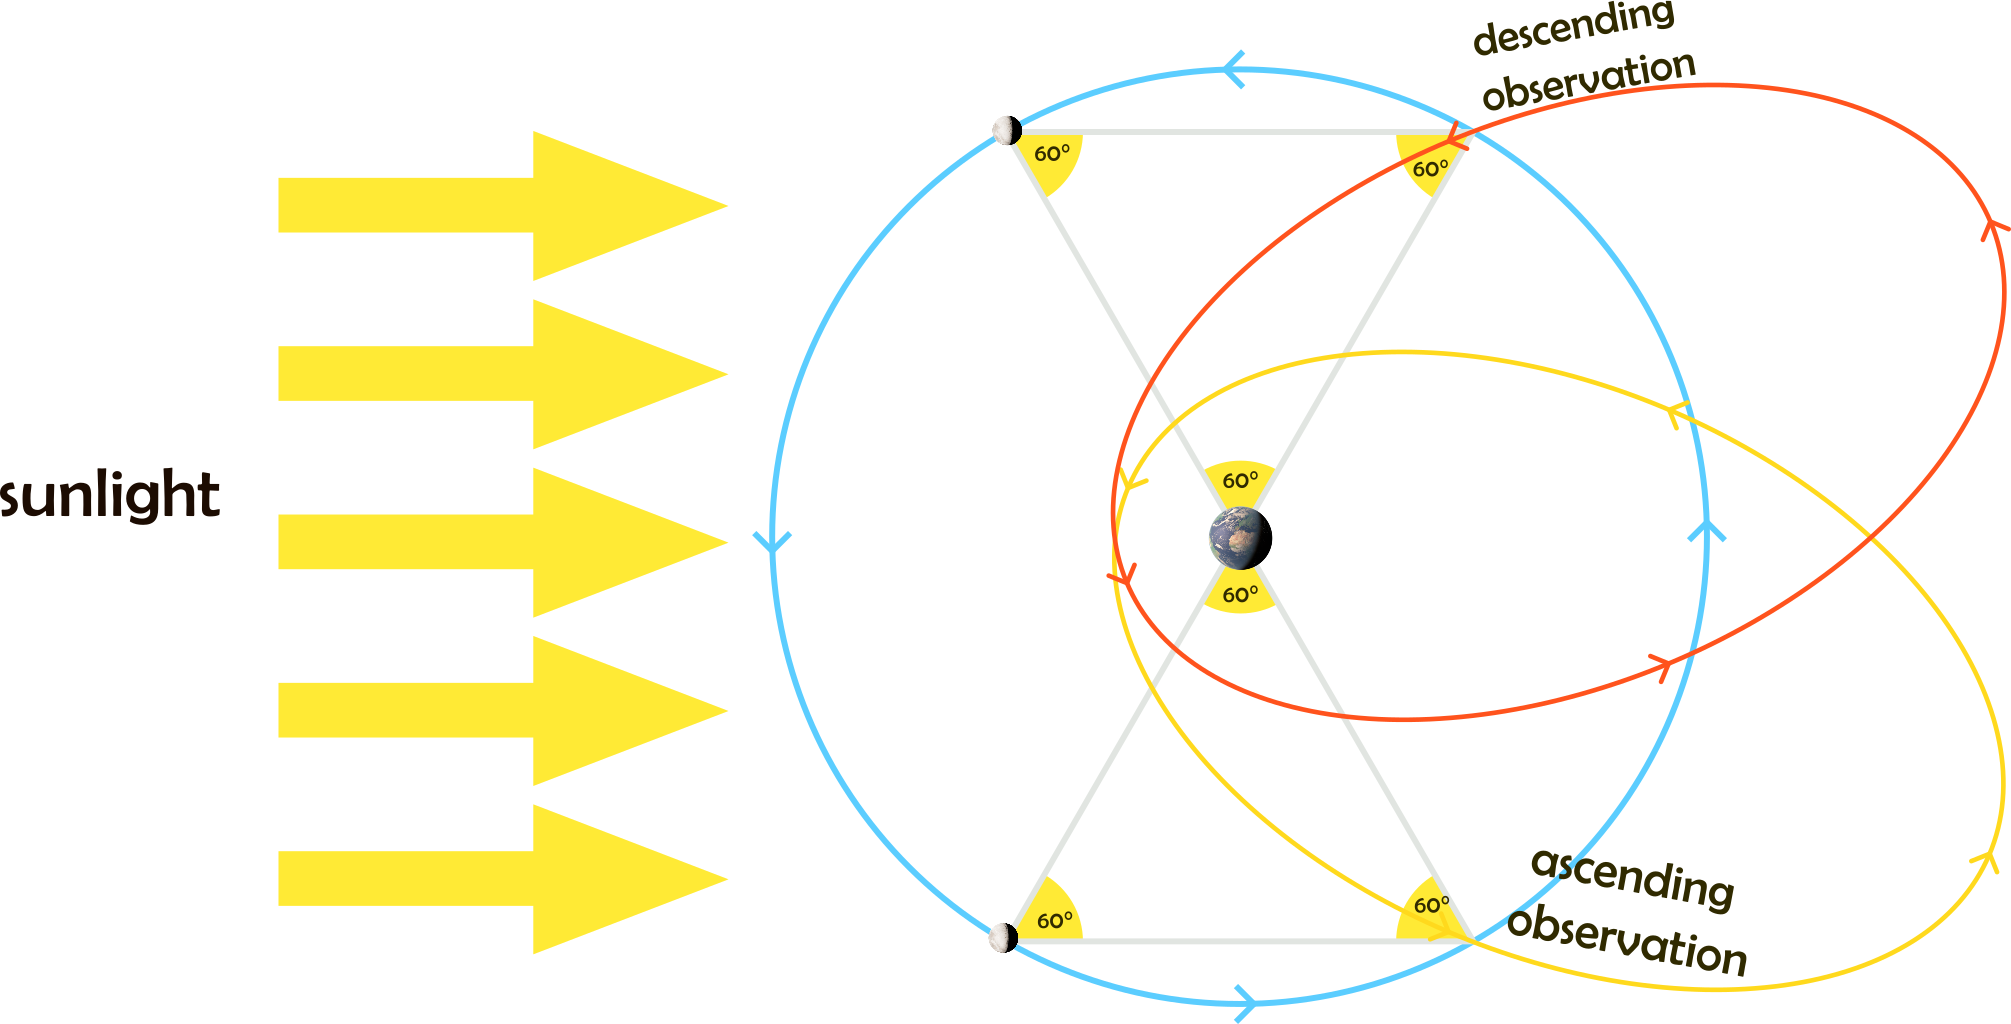
\includegraphics[width=18cm]{images/observations_main.png}
			\caption{orbites kepleriennes qui permettent de faire des observations aux points d'intérêt mentionné plus tôt}
		\end{figure}
		\\ \\
		Au fur et à mesure que le projet à avancé ,j'ai amélioré le modèle en prenant en compte de plus en plus de facteur comme l'excentricité et l'inclinaison de l'orbite de la Lune, la gravité de la Lune qui influence la dynamique du satellite ainsi que les variations de l'orbite de la Lune et de la Terre causé par l'influence gravitationnelle du Soleil sur le système Terre Lune (voir figure 3).
		\begin{figure}[h]
			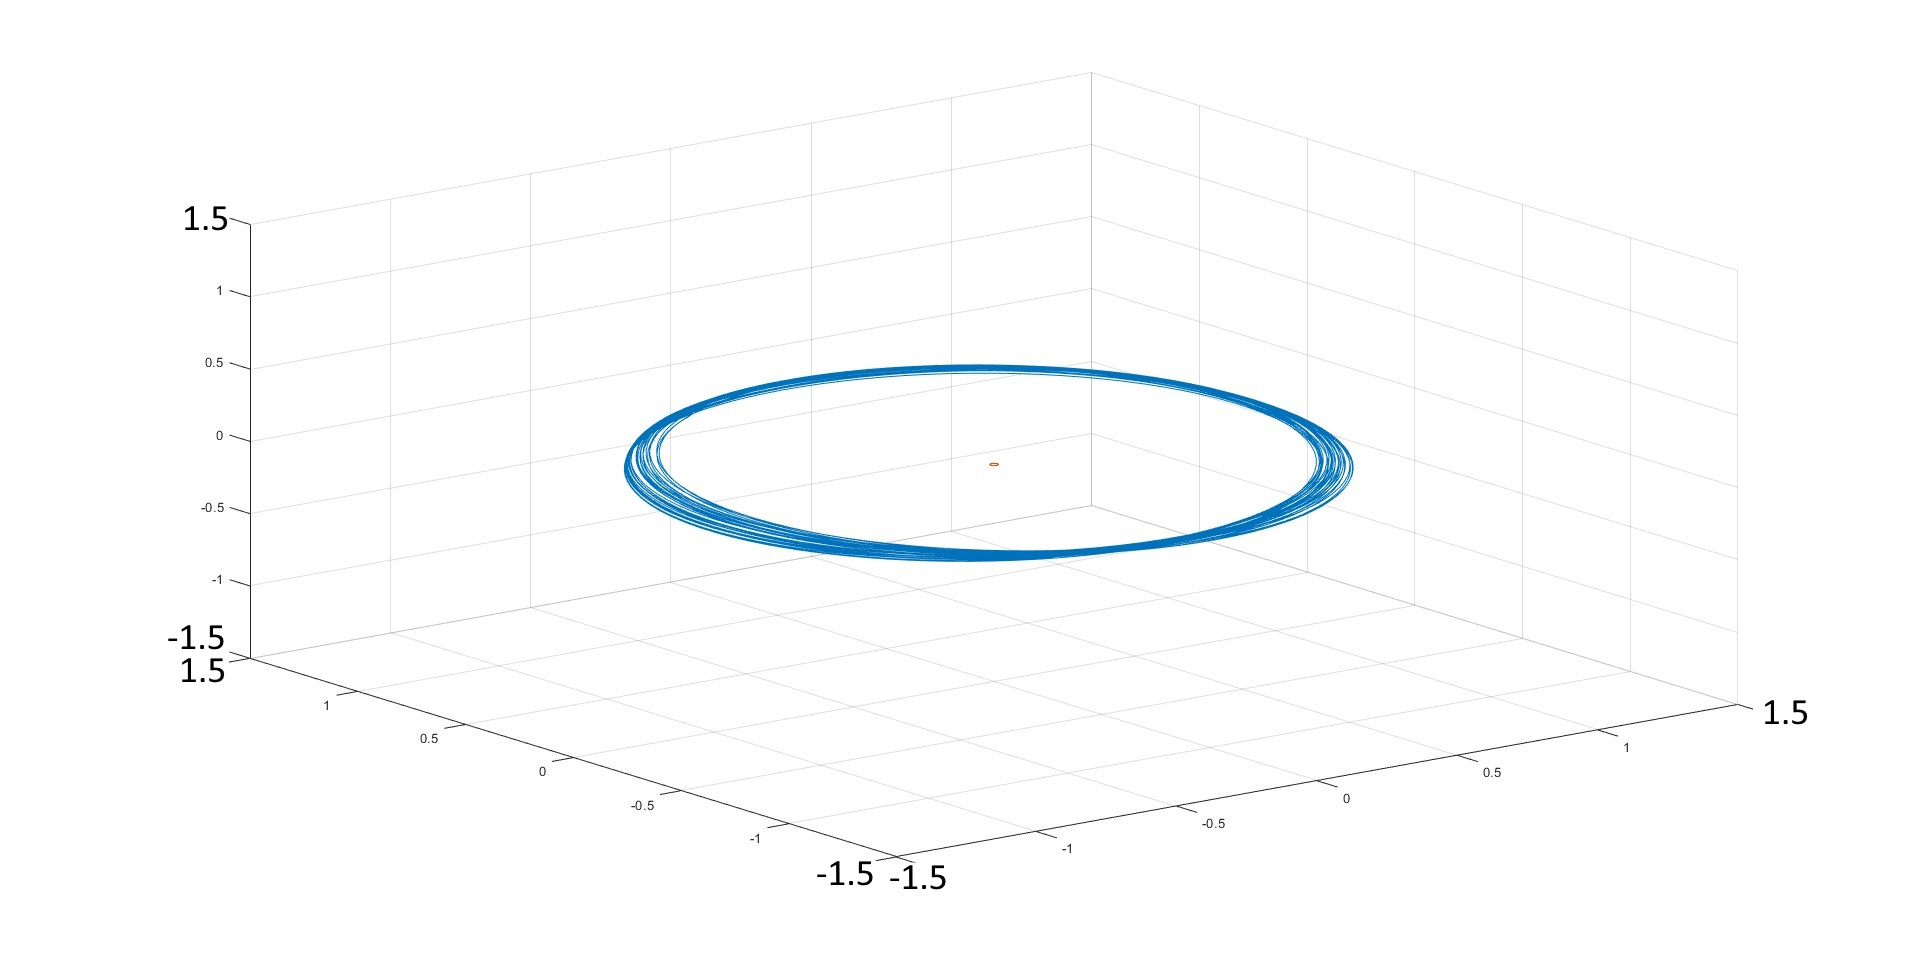
\includegraphics[width=1\textwidth]{images/moon_orbit.jpg}
			\caption{variation de l'orbite lunaire sur 2 ans}
		\end{figure}
		
		Aux termes du projet, le code MATLAB que j'ai réalisé avait d'une longueur approximativement 600 lignes et effectuait plusieurs opérations qui sont listées ci dessous: 
		
		\begin{itemize}
			\item simuler la dynamique du système à trois corps Soleil Lune Terre (l'influence de du système Terre-Lune sur le soleil est négligé);
			\item obtenir des approximation des emplacements des \glspl{Obs} optimales dans le but de trouver de bonnes conditions initiales à l'aide d'un modèle simplifié;
			\item optimiser les observations optimales pour chaque minimum trouvé à l'étape précédente
			\item obtenir des images graphiques et des fichiers csv contenant les données.
		\end{itemize}
		
		Le code à besoin en entrée de multiples informations sur la dynamique du problème dont la plupart des facteurs sont fournis directement dans le code. La partie venant de l'extérieur du code sont les positions et vitesses initiales du soleil de la Lune et de La Terre ainsi que quelques informations sur le nombre d'observations qu'il faut récupérer.
		Ce code pourrait être facilement adapté en une librairie qui pourra être ensuite incorporé dans des outils plus avancé par d'autres utilisateurs.
		Ce travail permis de confirmer l'intérêt des deux points de l'orbite lunaire qui semblait être les plus intéressants avec des temps d'observation situé entre 15 et 25 heures. En sachant qu'il y a deux observations de ce type pour chaque période synodique lunaire (environ 29.53 jours), cela permettrait de faire des observations pendant environs 2.8\% du temps (ou 1.4\% du temps en n'en faisant qu'une sur deux) de la mission ce qui est bien mieux que ce que l'on peut faire sur Terre (une observation de 10 minutes tout les 18 mois en moyenne soit environs 0.0015\% du temps).
		
		Le fait que les temps d'observation soit bien plus long aux points spécifiques où le satellite est lancé depuis la zone d'observation à la même vitesse que cette dernière m'a poussé à faire un test dans lequel le satellite étant toujours lancé à la même vitesse que la zone d'observation sans se soucier de sa période. Ce test à bien confirmé que les 2 observations trouvé précédemment sont bien les plus efficace mais a permis de mettre en évidence un $3^{eme}$ point de l'orbite lunaire aux alentour de $0^o$ (càd quand le Soleil, la Terre et la Lune sont alignés dans cette ordre). Cependant, cette troisième trajectoire n'est pas idéale car, en plus ne pas avoir une période similaire à celle de la lune, l'observation a lieu à proximité de la zone d'ombre de la Terre ce qui rendrait toutes observations impossible si la zone d'observation traversais l'ombre de la Terre. De plus, l'excentricité de l'orbite associée à cette trajectoire est aux alentour de 1 ce qui implique que le satellite pourrait facilement quitter le système Terre Lune ce qui pourrait être un problème en plus d'impliquer une énergie de mise en orbite initiale plus importante, c'est pourquoi cette observation n'a pas été étudiée dans l'étape suivante.
		\begin{figure}[h]
			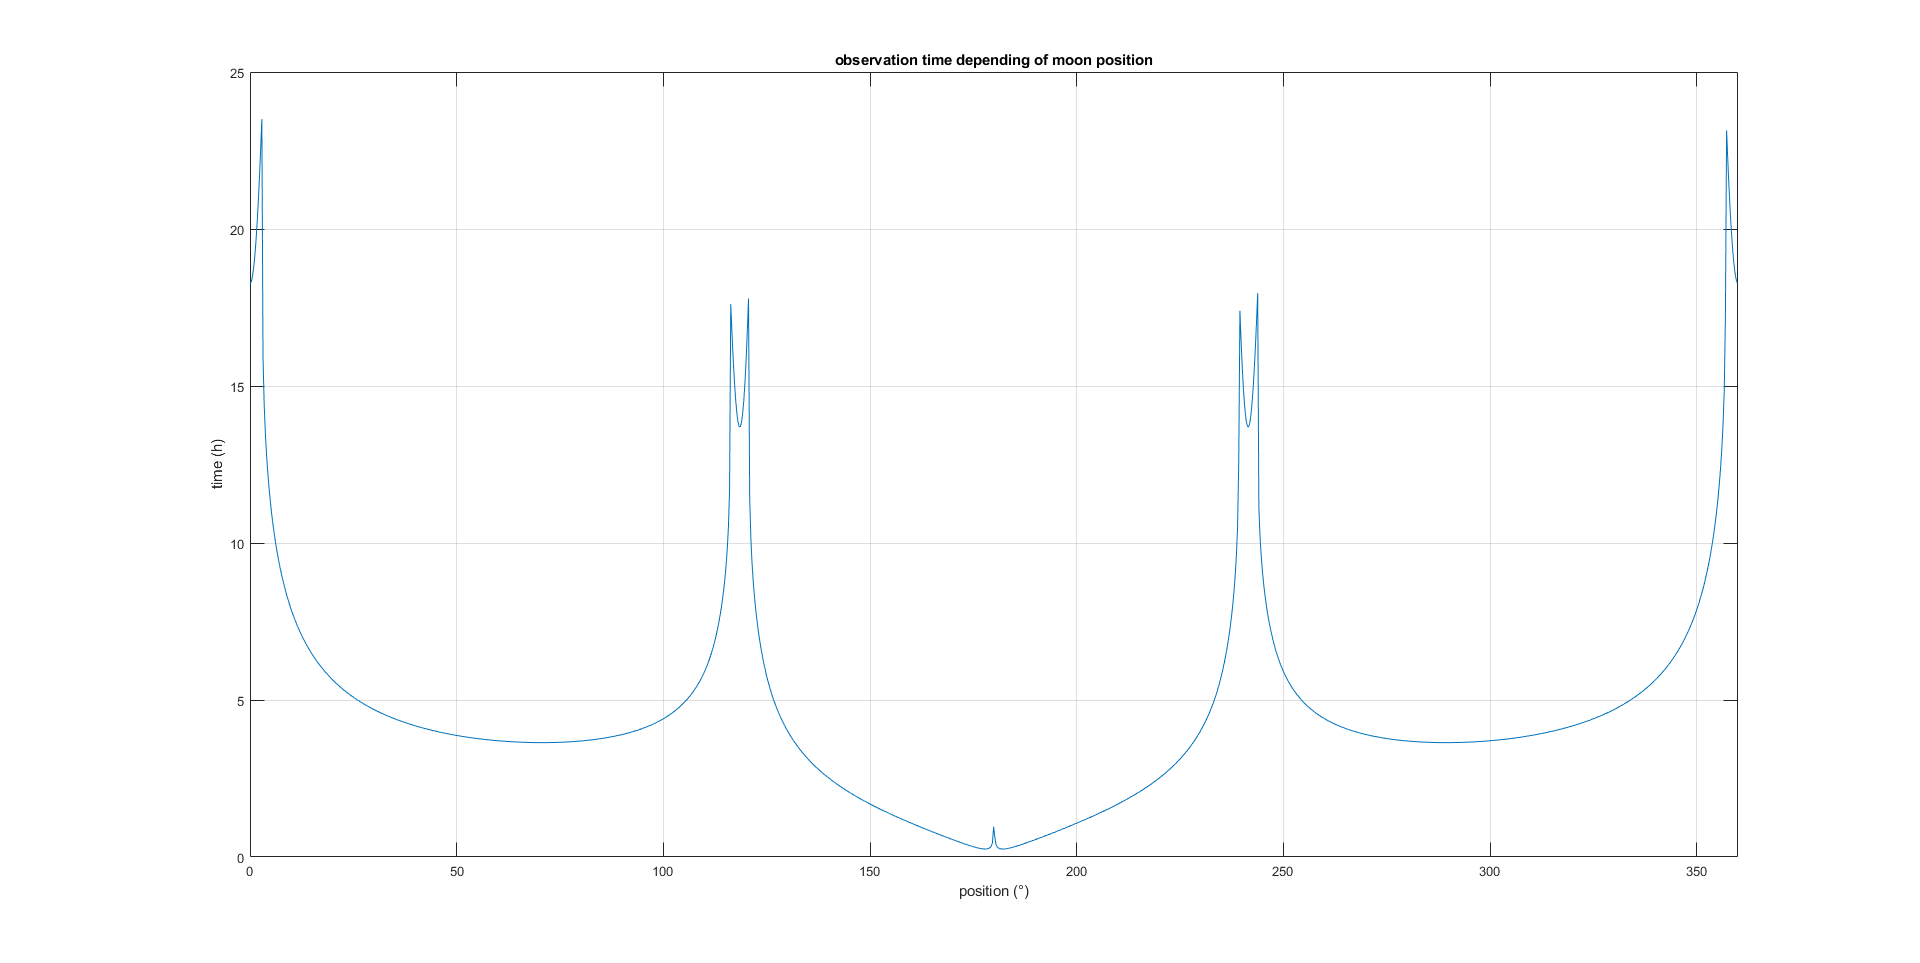
\includegraphics[width=1\textwidth]{images/observation_Obs.png}
			\caption{temps d'observation en fonction de l'anomalie vraie de la Lune}
		\end{figure}
		
		\subsection{Contrôle optimal}
		
		L'étape suivante consistait à calculer la trajectoire du satellite pour joindre les différentes observations.
		pour cela j'ai utilisé une librairie en Julia permettant de résoudre des problèmes de contrôle optimal, l'idée était de calculer tout les transferts possible entre différentes observations.
		
		On utilise la même méthode que précédemment pour calculer la position de la Terre et de la Lune, cependant on ajoute un contrôle à la dynamique du satellite ainsi qu'un paramètre supplémentaire pour la masse :
		
		$$
		\begin{bmatrix}
			\dot{\overrightarrow{R_{s}}}\\
			\dot{\overrightarrow{V_{s}}}\\
			\dot{m_{s}}
		\end{bmatrix} =\begin{bmatrix}
			\overrightarrow{V_{s}}\\
			G_{m}(R_s,R_m)+G_{t}(R_s,R_t)+u\frac{M_{t}}{m}\\
			-Q\|u\|
		\end{bmatrix}
		$$
		
		L'état initial du satellite est fixé et l'état final l'est également à l'exception de la masse qui est laissé libre (mais contrainte supérieure aux chargement du satellite). Les temps de départ est d'arrivé sont également fixés.
		L'objectif est de minimiser l'énergie cinétique lors d'un transfert calculé avec l'équation de coût suivante :
		
		$C=\int_{t_0}^{t_f}\frac{1}{2}\|u\|^2dt$
		
		Voici ci dessous quelques schémas illustrant les liens entres les orbites de départ et d'arrivé étudié, le transfert entre une observation descendante à ascendante (en haut à droite) demande de trop grand changement d'orbite en un temps trop court (environs 10 jours). Le passage d'une observation descendante à une observation ascendante en sautant un mois (en bas à gauche) est très facile car les orbites se retrouvent quasiment alignées. Cependant le transfert inverse (en bas à droite) demande au contraire plus d'énergie car les orbites se sont encore plus éloignés au lieu de se rapprocher. De manière générale les transferts entre deux observations du même type demande une quantité relativement faible d'énergie.
		\begin{figure}[H]
			\includegraphics[width=0.5\textwidth]{images/1in2obs.png}
			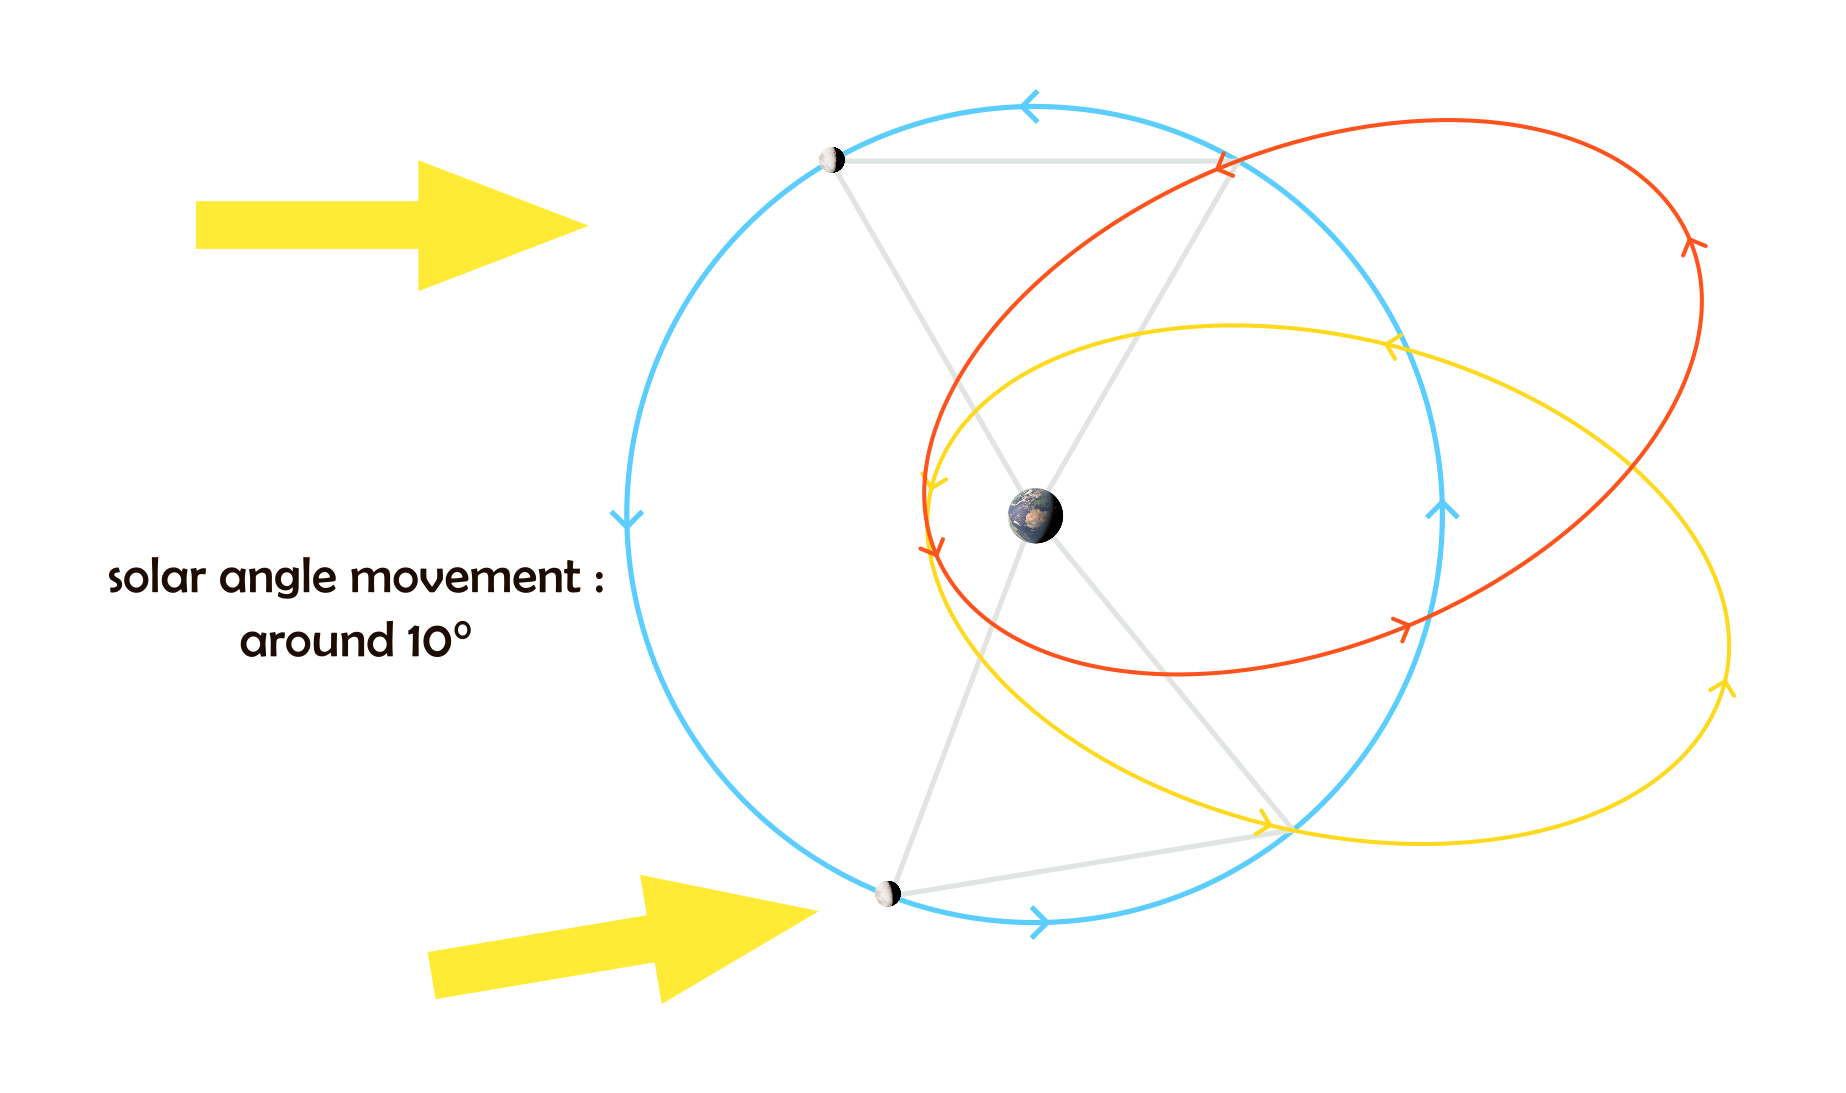
\includegraphics[width=0.5\textwidth]{images/odd_to_even.png}
			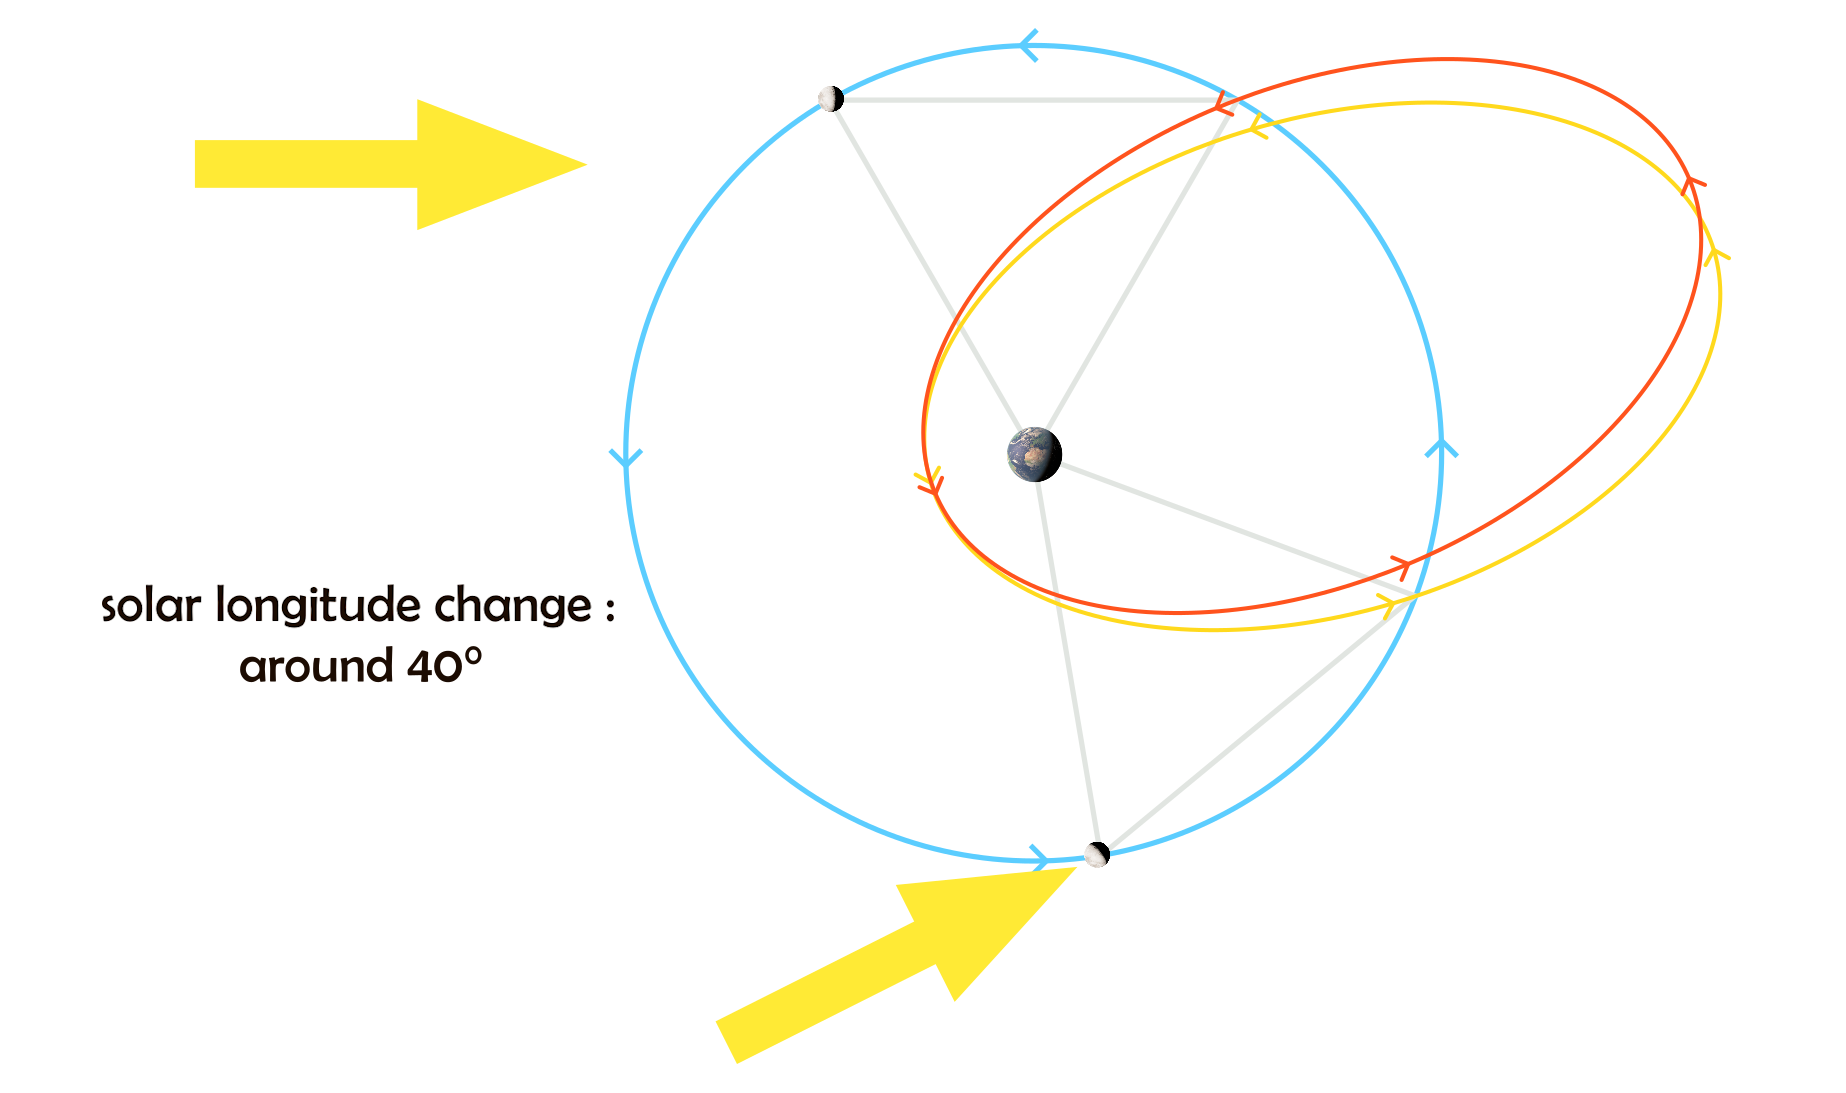
\includegraphics[width=0.5\textwidth]{images/1in3_obs.png}
			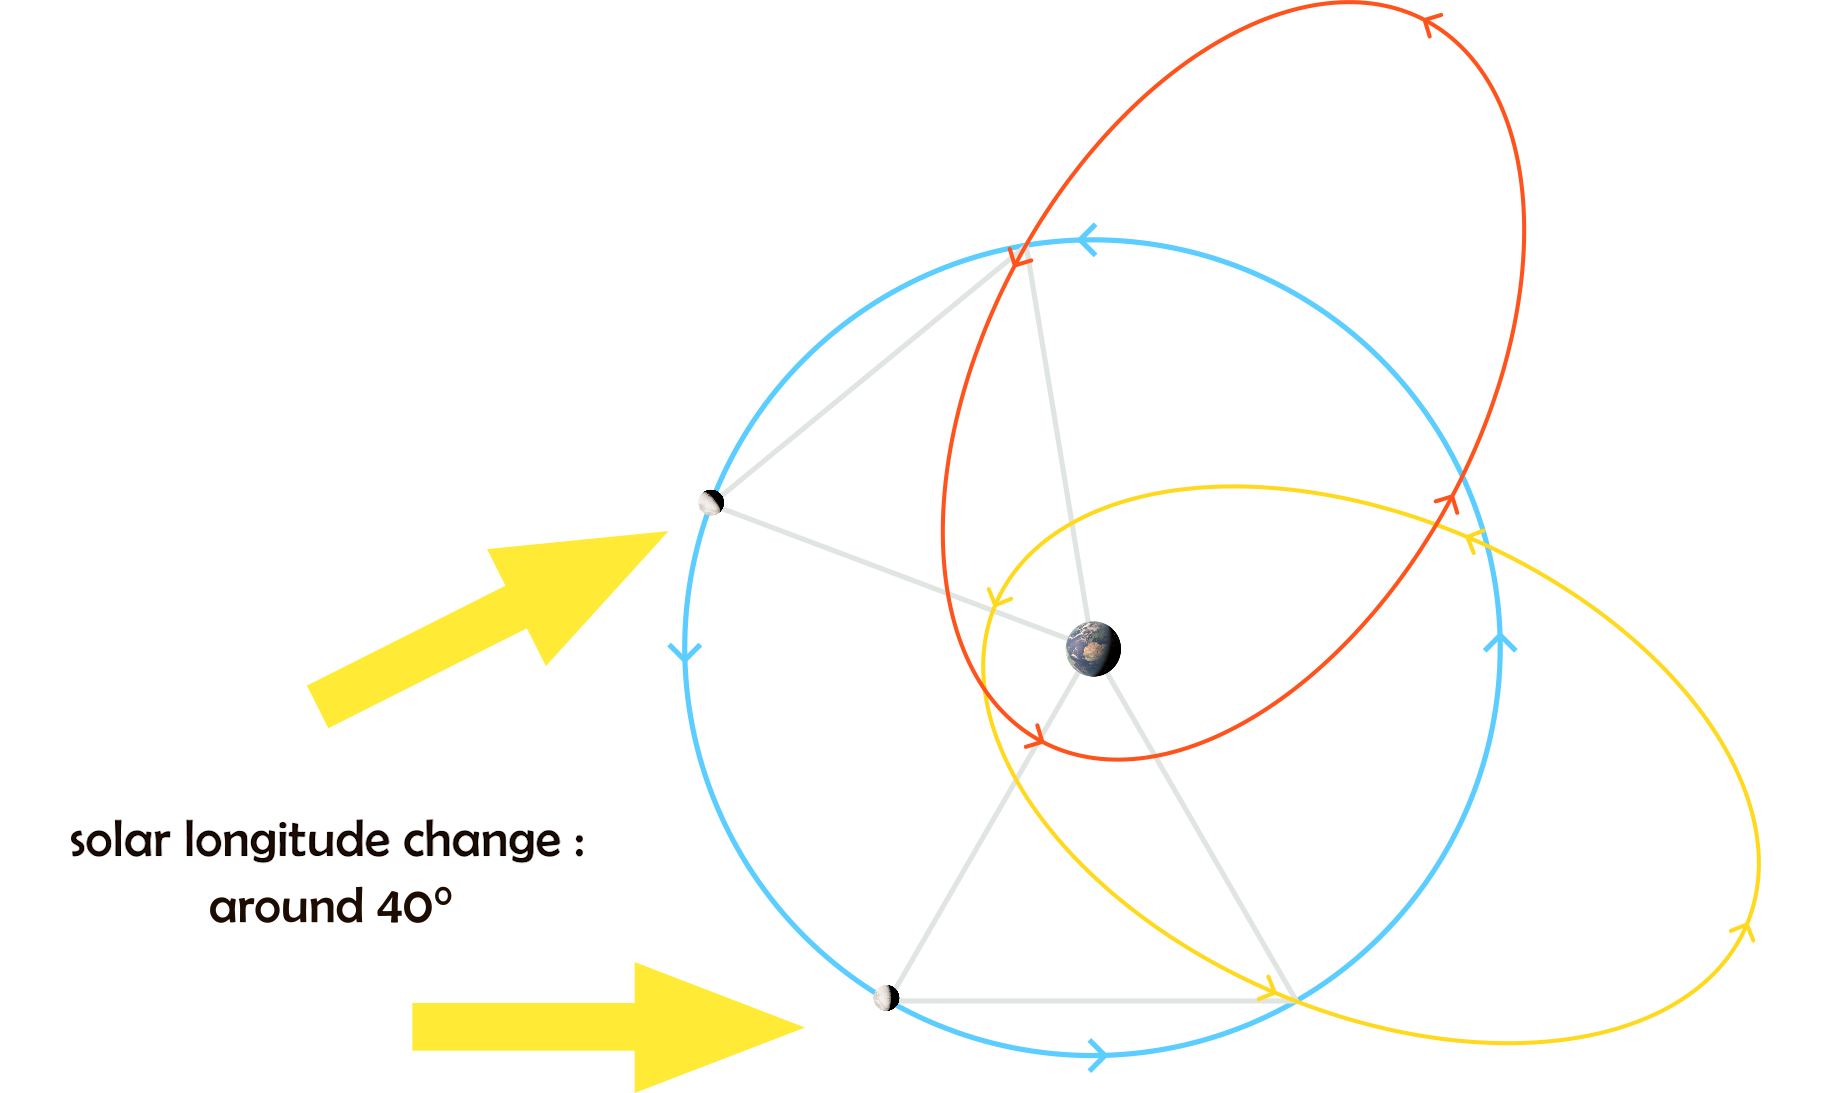
\includegraphics[width=0.5\textwidth]{images/1in3_bad.png}
		\end{figure}
		
		De manière générale les accélérations maximales nécessaires pour ces transferts se sont avérés trop élevés pour des voiles solaires, c'est à partir de ce moment là que l'option des voiles solaires a été écarté au profit des moteurs ioniques.	
		%Après avoir implémenté une version simplifiée du problème des voiles solaires (poussée faible dans n'importe quelle direction), il se trouve que les accélérations demandées semblaient trop élevées pour utiliser une voile solaire, l'option d'utiliser un satellite à poussée faible a donc été sélectionné.
		
		Concernant les transferts, j'ai effectué une analyse des résultats qui m'ont permis de sélectionner 2 scénarios possible de mission dans lesquels un satellite effectue une observation sur 2 en utilisant une poussée faible.
		
		Suite à ces premiers calculs j'ai mis à jour le programme pour prendre en compte l'équation de la masse, j'ai utilisé comme moteur le RIT-10 evo. Ce nouveau code à ensuite été raffiné pour effectuer les opérations suivantes : 
		
		\begin{itemize}
			\item simuler la dynamique du système à trois corps Soleil Lune Terre (l'influence de du système Terre-Lune sur le soleil est négligé);
			\item définir et résoudre un modèle de contrôle optimal de transfert avec bord fixé en minimisant l'énergie dépensée.
			\item écrire les résultats dans des fichiers csv.
		\end{itemize}
		
		\subsection{Analyse des résultats}
		
		A plusieurs reprises durant ce stage j'ai du commenter des résultats de calculs, j'ai du rechercher les raisons et les causes qui ont mené à certain résultat inattendus ainsi que de déduire des potentiels calculs supplémentaire ou les prochaines étapes du projet. Pour commencer j'ai utilisé les résultats du solver qui trouvait les plus long temps d'observations pour isoler des les points les plus intéressants  (\gls{AscObs} et \gls{DesObs}) pour faire des observations. Suite à ces analyse j'en ai conclu que ce qui semblait le plus intéressant était d'optimiser les observations indépendamment les unes des autres puis de chercher par la suite des trajectoire de transfert qui permettrait de passer d'une orbite à l'autre.
		
		%J'ai également du faire de choix en fonctions de ces résultat. J'ai par exemple remarqué qu'en prenant une période de révolution plus courte pour le satellite ( de l'ordre de $0.92$ période lunaire au lieu de $1$) les temps d'observation obtenue était plus court. Je pense que la cause de ces résultat vient du fait que la contrainte de vitesse lié à la période fixée du satellite est de trop, cependant donner au satellite la liberté d'avoir n'importe quelle vitesse en partant des optimums trouvé avec le modèle simplifié donne de très mauvais résultat. J'ai donc décidé d'optimiser d'abord avec la norme de vitesse fixé par la période du satellite (fixé à $0.92$) puis de résoudre à nouveau avec un modèle modifié laissant la vitesse libre en prenant comme condition initiale le résultat de l'algorithme précédent. Il est probable qu'il faillent remplacer le modèle simplifié par un autre plus performant. Un qui prendrait en compte le temps d'observation en fixant la vitesse de l'objet à la vitesse de la zone d'observation comme dans la figure 2 par exemple. Mais la forme assez complexe des optimums (deux pics très rapproché) et le fait que les observations des résultats ont rarement montré des trajectoire à vitesse nulle au centre de la zone (les vitesses sont souvent nulles près des bord de la zone) ont fait que je n'ai pas eu le temps d'implémenter un autre modèle.
		
		Ensuite j'ai du analysé les résultats de mon second code fait en Julia pour essayé de comprendre pourquoi les accélérations maximale des transferts ne diminuait pas même en faisant des transferts sur plus longtemps.
		Il s'avère que, si l'on considère un modèle simplifié d'une Lune et d'une Terre avec une orbite circulaire sur le même plan, les orbites d'observations sont sensiblement les mêmes avec pour unique différence une rotation autour du vecteur normal au plan écliptique. Cette rotation est proportionnelle aux temps entre deux observation. Cela signifie que plus deux observations sont éloigné plus il faudra faire tourner l'orbite d'observation sur un grand angle ce qui explique que la les accélérations maximales ne diminuaient pas. Effectuer un transfert sur une observation deux fois plus lointaine dans le temps nécessite de faire tourner l'orbite d'observation deux fois plus loin également. C'est cette conclusion suggérant qu'il y a un seuil d'accélérations minimal que doit atteindre le satellite pour effectuer un nombre important d'observations par an qui à mené à l'abandon des voiles solaires au profit d'un moteur à poussée faible.
		
		\begin{figure}[H]
			\centering
			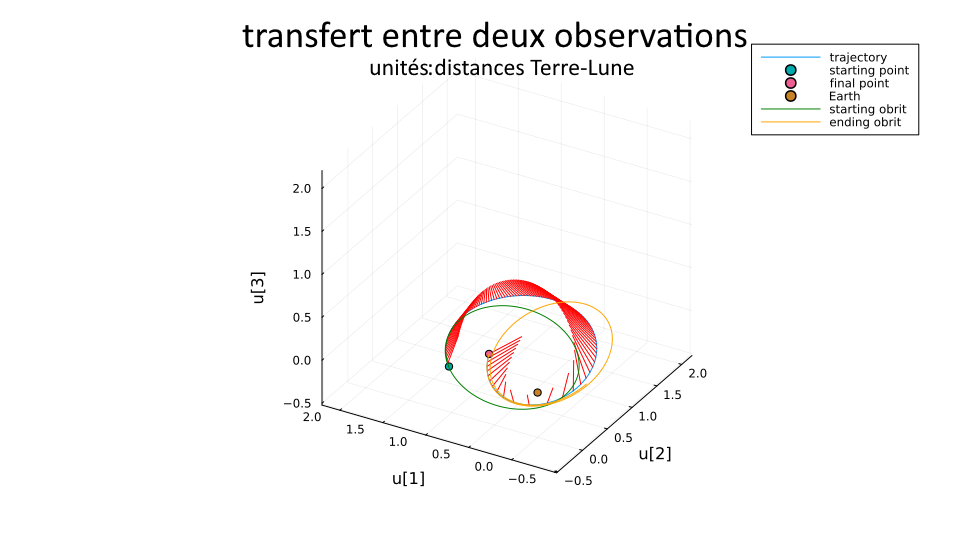
\includegraphics[width=0.9\linewidth]{images/Transfert_23_25}
			\caption{trajectoire typique suivie par le satellite lors d'un transfert}
		\end{figure}
		\begin{figure}[H]
			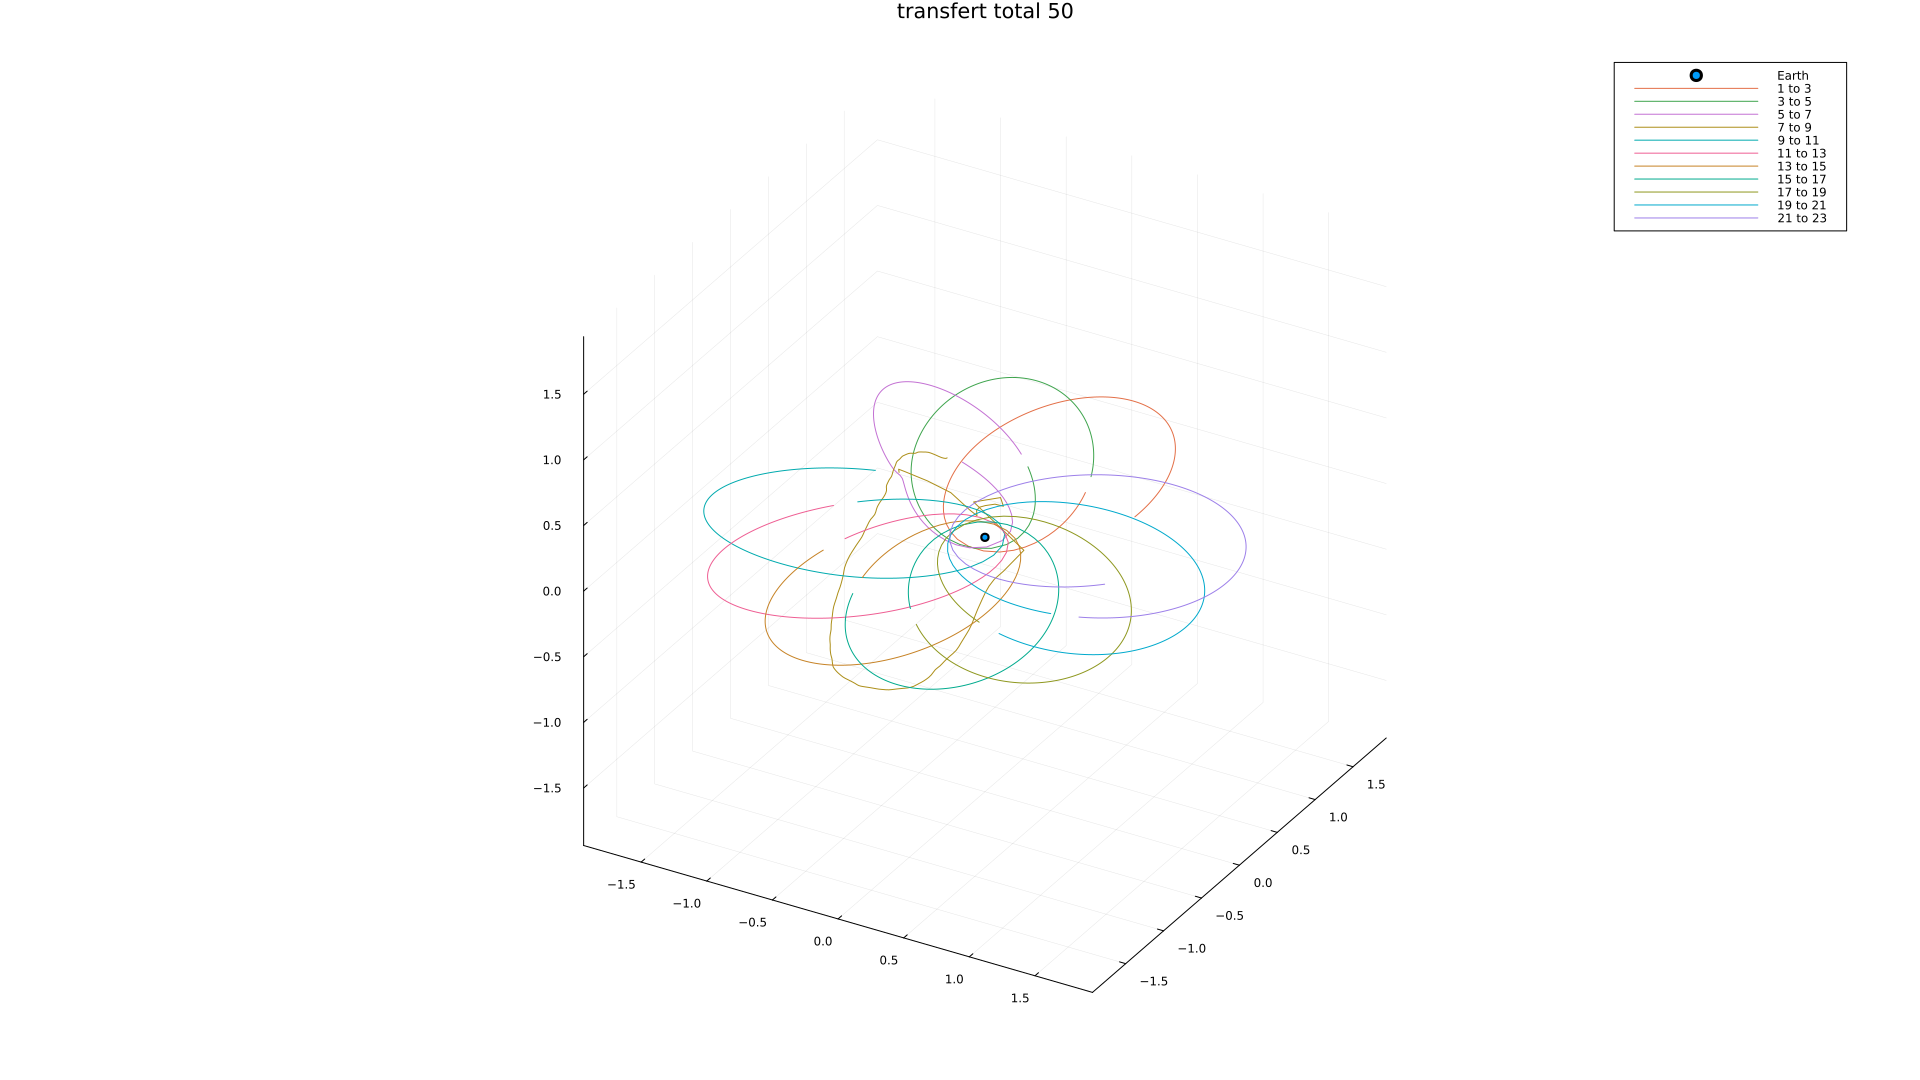
\includegraphics[width=0.9\linewidth]{images/All_transfert_odd_48_50}
			\caption{tous les transferts du premier scénario de la première année mis les uns à la suite des autres, on peut voir que l'orbite tourne sur elle même en quelque sorte}
		\end{figure}
		\newpage
		\section{Conclusion}
		\subsection{Compétences acquises}
		Pour conclure ce stage m'a permis d'obtenir de nombreuses compétences.
		 J'ai eu l'occasion de maîtriser les bases du contrôle optimal. Ce stage m'a également permis de mettre en application ces connaissances en utilisant une librairie permettant de résoudre des problèmes de ce type.
		
		J'ai également renforcé mes compétences en programmation en apprenant un nouveau langage de programmation : le Julia qui est un langage utilisé en recherche pour le calculs scientifique et la résolution numérique de problème.J'ai également grandement amélioré mes connaissances dans le langage de programmation Matlab qui est lui aussi un langage utilisé pour la résolution numérique de problèmes.
		
		Le fait de programmer en deux langages différent m'a forcé faire transiter les résultats d'un programme à l'autre en utilisant des fichiers csv ce qui m'a permis de faire des applications plus propres et à renforcé mes capacité à créer des codes pouvant être inclus et utilisés dans d'autres applications que celles pour lesquelles ils avaient été initialement programmés.
		
		J'ai eu également l'occasion d'écrire un compte-rendu de projet (qui n'est pas ce rapport de stage) intégralement en Anglais ce qui, en plus de renforcé mes compétences en Anglais, m'a permis de devenir plus doué dans la rédaction de rapports scientifiques en vue de publication.
		
		\subsection{Travail réalisé}
		
		Durant ce stage j'ai produit de nombreux résultat qui pourront être réutilisé par d'autres personnes à l'avenir. on compte permis ces résultats : 
		\\ \\
		Premièrement j'ai produits deux programme, un programme réalisé avec le langage MATLAB qui calcule toutes les observations faisable sur un intervalle de temps, ce programme prends en entrée plusieurs fichiers CSV contenant des paramètre sur le code à exécuter ainsi que les positions initiales de la Terre la Lune et le Soleil. Ce code produits comme résultat plusieurs ficheirs CSV correspondant aux temps de départ, et de fin d'observation ainsi que les positions et vitesses qu'aurait un objet effectuant ces observations à l'entrée et la sortie de la zone d'observation.
		
		J'ai également produit un code en Julia qui prends en entrée les résultats du code précédent (dans le même format de fichier) et calcule des trajéctoire avec contrôle qui permettent de relier des observations de sorties et des observations. ce programme donne en sortie de nombreuses données de résultats sous le format CSV.
		
		Ces deux programmes donnent aussi chacun des graphiques et des images qui permettent d'avoir un support visuel des résultats.
		
		\subsection{Possibilités pour aller plus loin}
		Si mon stage avait duré plus longtemps, j'aurais pu continuer à explorer les possibilité pour des missions d'observations de la Lune en essayant d'améliorer mes codes, j'aurais pu aussi étudier des possibilité que j'ai laisser de côte comme la troisième observations qui pourrait peut être fournir des scénario viable avec une voile solaire. J'ai aussi manqué de temps pour vérifier certaines des observations que j'ai durant ce stage, si j'avais eu plus de temps, j'aurais pu faire de nombreux tests, comparatifs et vérification qui permettrons certainement de mieux comprendre les variables importantes du problème, notamment essayer d'expliquer ce qui cause l'existence de ces pics de temps élevé (\gls{AscObs} et \gls{DesObs}) ce qui pourrait permettre de créer un modèle simplifié plus efficace que celui utilisé actuellement.
		
		\vfill
		
		\section{Glossaire}
		
		\printglossaries
		
		%a placer au bon endrois
		
		
\end{document}